\documentclass[a4paper]{article}

%%%%%%%% CREATE DOCUMENT STRUCTURE %%%%%%%%
%% Language and font encodings
\usepackage[english]{babel}
\usepackage[utf8x]{inputenc}
\usepackage[T1]{fontenc}
%\usepackage{subfig}

%% Sets page size and margins
\usepackage[a4paper,top=3cm,bottom=2cm,left=2cm,right=2cm,marginparwidth=1.75cm]{geometry}

%% Useful packages
\usepackage{amsmath,amssymb}
\usepackage{graphicx}
\usepackage[colorinlistoftodos]{todonotes}
\usepackage[colorlinks=true, allcolors=blue]{hyperref}
\usepackage{caption}
\usepackage{subcaption}
\usepackage{sectsty}
\usepackage{apacite}
\usepackage{float}
\usepackage{titling} 
\usepackage{blindtext}
\usepackage[square,sort,comma,numbers]{natbib}
\usepackage[colorinlistoftodos]{todonotes}
\usepackage{xcolor}
\definecolor{darkgreen}{rgb}{0.0, 0.4, 0.0}
\usepackage{graphicx}
\newcommand{\norm}[1]{\left\lVert#1\right\rVert}
\DeclareMathOperator{\R}{\mathbb{R}}
\DeclareMathOperator{\E}{\mathbb{E}}

\usepackage{listings}
\usepackage{xcolor}

\definecolor{codegreen}{rgb}{0,0.6,0}
\definecolor{codegray}{rgb}{0.5,0.5,0.5}
\definecolor{codepurple}{rgb}{0.58,0,0.82}
\definecolor{backcolour}{rgb}{0.95,0.95,0.92}

\lstdefinestyle{mystyle}{
	backgroundcolor=\color{backcolour},   
	commentstyle=\color{codegreen},
	keywordstyle=\color{magenta},
	numberstyle=\tiny\color{codegray},
	stringstyle=\color{codepurple},
	basicstyle=\ttfamily\footnotesize,
	breakatwhitespace=false,         
	breaklines=true,                 
	captionpos=b,                    
	keepspaces=true,                 
	numbers=left,                    
	numbersep=5pt,                  
	showspaces=false,                
	showstringspaces=false,
	showtabs=false,                  
	tabsize=2
}

\lstset{style=mystyle}
 



%%%%%%%% DOCUMENT %%%%%%%%
\begin{document}

%%%% Title Page
\begin{titlepage}

\newcommand{\HRule}{\rule{\linewidth}{0.5mm}} 							% horizontal line and its thickness
\center 
 
 
% University


\includegraphics[width=0.15\textwidth]{images/kth_logo.png}\\[0.5cm] 	% University logo

\textsc{\LARGE KTH Royal Institute of Technology}\\[1cm]

% Document info
\textsc{\Large Deep Learning in Datascience}\\[0.2cm]
\textsc{\large DD2424}\\[1cm] 										% Course Code
\HRule \\[0.8cm]
{ \huge \bfseries Assignment 2}\\[0.7cm]								% Assignment
\HRule \\[2cm]
\large
\emph{Authors:}\\
Ali Banaei Mobarak Abadi\\[1.5cm]													% Author info
{\large \today}\\[5cm]

\vfill 
\end{titlepage}

%%\begin{abstract}
%%Your abstract.
%%\end{abstract}

%%%% SECTIONS
%% Section 1
\section{Checking the gradients}

After implementing the needed functions, we had to test the computed gradients using the back-propagation algorithm using the numerical estimation of the gradient. First, the initialization of the weight and bias matrices were changed. The initial values are selected uniformly from -2 to 2. By this way of initializing, the weights will have relatively big values, and this leads to first amplifying potential errors and second big gradient values, which enables us to compare them only using the absolute value of the difference. The results were as follows.

\begin{lstlisting}
	for W1: Max:0.7817716323188506, mean:-0.00980110914407343, std:0.17618794810131944 
	for W1 error: Max:1.4683249884739347e-05, mean:1.0347053330027051e-05, std:5.720060851032624e-07
	for W2: Max:13.493227888830006, mean:0.00019611783500295132, std:2.7529251052726416 
	for W2 error: Max:0.0036512718726414706, mean:0.0001696644400953728, std:0.00045737611577545433
	for b1: Max:0.3236899010516936, mean:0.07040882082947064, std:0.126665873714558 
	for b1 error: Max:1.2523320971694063e-06, mean:2.4300402196618996e-07, std:2.7540197710057374e-07
	for b2: Max:0.284773650491843, mean:2.02817318495363e-07, std:0.1318978074614518 
	for b2 error: Max:6.511011487186913e-07, mean:2.0601960361160687e-07, std:2.2085068043956378e-07
\end{lstlisting}

As we can see, the error value compared to the gradient values is very small and is due to the numerical estimation and floating-point calculation error. So, we can proceed without worrying about the correctness of the gradients.

\section{Overfitting the network on small dataset}

In the next step, in order to make sure the network is learning properly, a small dataset containing only 100 samples with no regularization on the network were utilized. If we are performing the learning correctly, the network must overfit the training data meaning that we will see a very small value for training loss while the validation loss remains big. As shown below, the overfitting clearly happened.

\begin{lstlisting}
	epoch 199/200, trainingloss:0.0013889283351083822, training cost:0.0013889283351083822, validation loss:10.279636223892174, validation cost:10.279636223892174
\end{lstlisting}


\section{Cyclic learning rate}

Now, it is time to implement the cyclic learning rate. As can be found in the code, the learning rate scheduler function is used during the training. First, the scheduler was tested by plotting the returned learning rate over iterations which can be found in \autoref{fig:cycle}.

\begin{figure}[h]
	\centering
	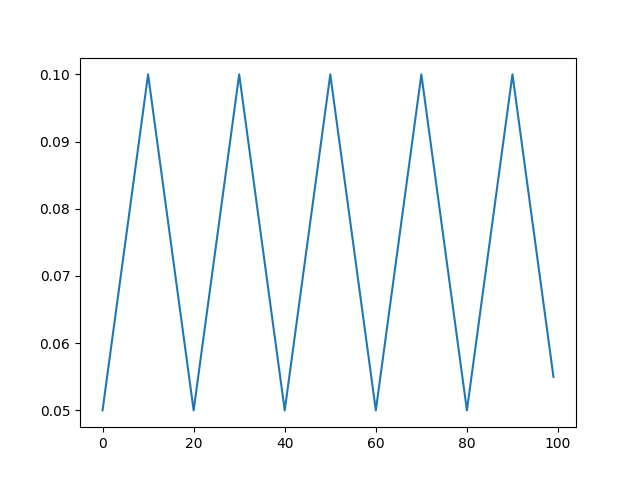
\includegraphics[width=0.5\linewidth]{images/scheduler.png}
	\caption{Learning rate in each iteration from 0 to 100 with $lr_{max}=0.1$, $lr_{min}=0.05$ and $n_s=10$}
	\label{fig:cycle}
\end{figure}

After checking the scheduler, implemented MLP was trained on 10000 samples with the specified settings of hyperparameters in the lab instructions. Loss function, cost, and accuracy during training can be found in \autoref{fig:ex3}. Note that since the recording of these values was done in each iteration, the graphs have more fluctuation compared to the ones in the instructions.  The graphs have the same overall characteristics and appearance as in the instructions. The trained network could classify the thest samples with an accuracy of \%43.2 .


\begin{figure}[h]
	\centering
	\begin{subfigure}{0.3\textwidth}
		\centering
		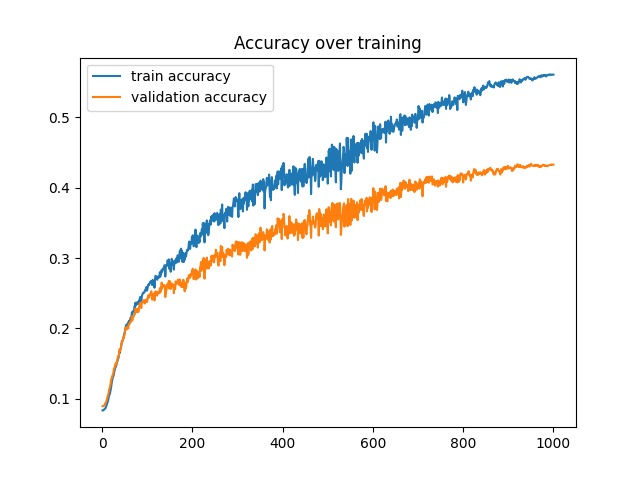
\includegraphics[width=\linewidth]{images/1000_it_default_acc.png}
		\caption{Accuracy}
	\end{subfigure}
	\begin{subfigure}{0.3\textwidth}
		\centering
		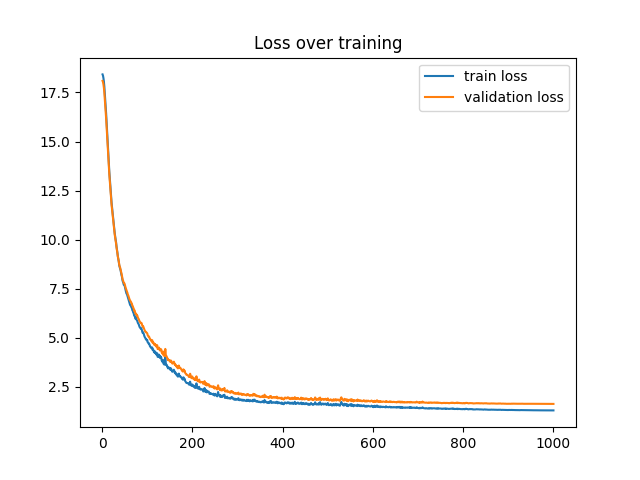
\includegraphics[width=\linewidth]{images/1000_it_default_loss.png}
		\caption{Loss}
	\end{subfigure}
	\begin{subfigure}{0.3\textwidth}
		\centering
		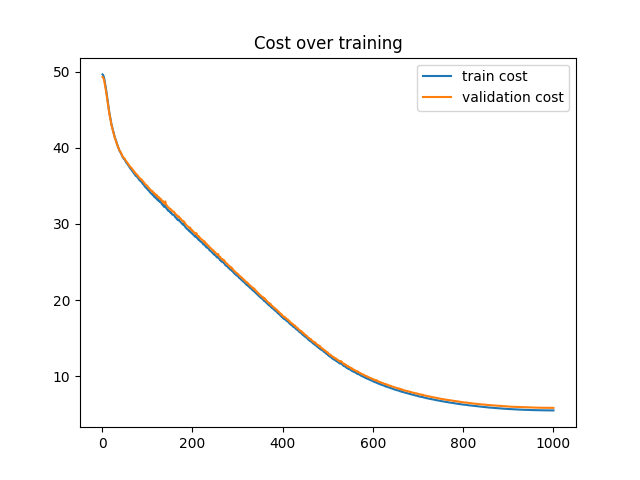
\includegraphics[width=\linewidth]{images/1000_it_default_cost.png}
		\caption{Cost}
	\end{subfigure}
	\caption{Training of the network with the settings of Exercise 3.}
	\label{fig:ex3}
\end{figure}



\autoref{fig:ex4} depicts the same metrics for training a network using the settings of exercise 4. As we see, there is a gap between training and validation curves. This gap which seems increasing, can be a sign of potential overfitting if we do not use more data or other regularisation techniques. The resulting network reached the accuracy of \%46.9 over the test set.



\begin{figure}[h]
	\centering
	\begin{subfigure}{0.3\textwidth}
		\centering
		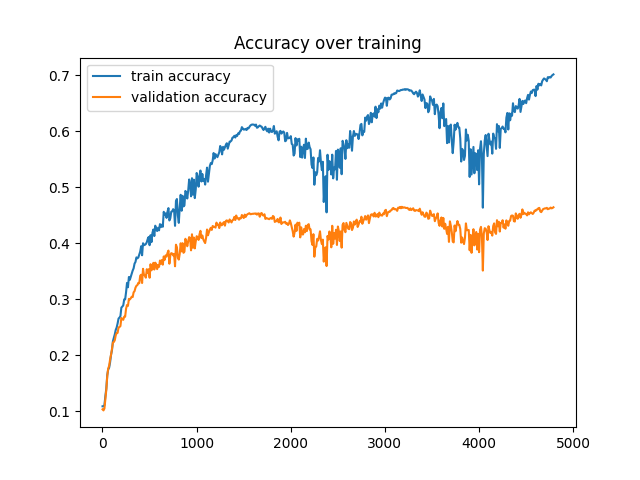
\includegraphics[width=\linewidth]{images/exercise4_acc.png}
		\caption{Accuracy}
	\end{subfigure}
	\begin{subfigure}{0.3\textwidth}
		\centering
		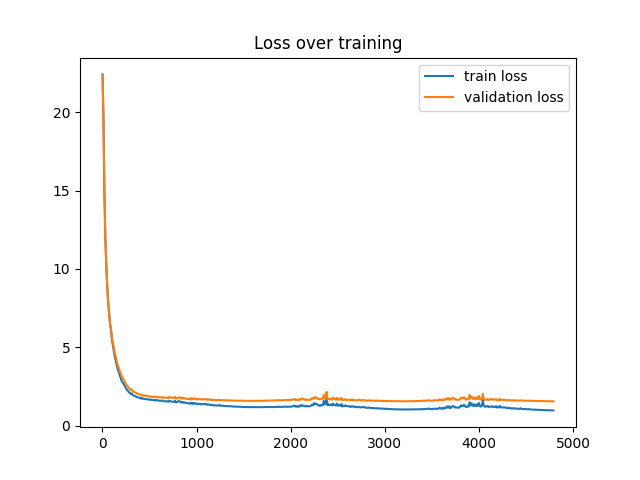
\includegraphics[width=\linewidth]{images/exercise4_loss.png}
		\caption{Loss}
	\end{subfigure}
	\begin{subfigure}{0.3\textwidth}
		\centering
		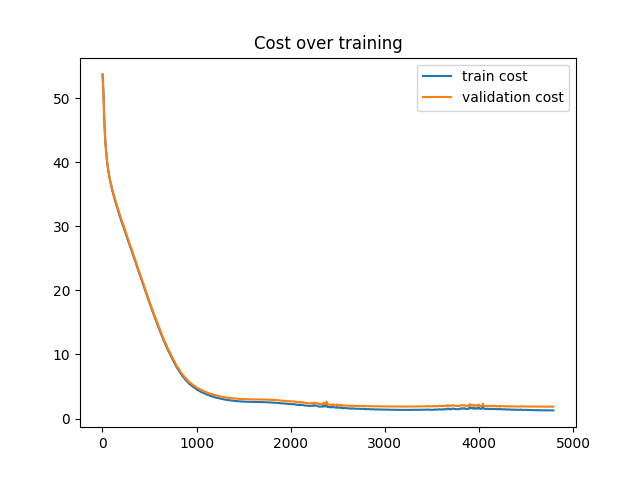
\includegraphics[width=\linewidth]{images/exercise4_cost.png}
		\caption{Cost}
	\end{subfigure}
	\caption{Training of the network with the settings of Exercise 4.}
	\label{fig:ex4}
\end{figure}

\section{Fine-tuning $\lambda$ and final model}
In order to find the best performing lambda, a two step search was performed. In the first step or the coarse search which we search a wider range of values for lambda. The model was trained for 4 epochs on all training data and the final accuracy over validation set was measured. Note that training the model for longer times could lead to more accurate estimation of the effect of each hyperparameter, but because of compatational limitations, 4 iteration over all the training data was used. The results of this search can be found in \autoref{tab:coarse}.

\begin{table}[h]
	\centering
	\caption{Coarse search of lambda value for L2 regularization.}
	\label{tab:coarse}
	\begin{tabular}{|l|l|} 
		\hline
		Lambda           & Accuracy  \\ 
		\hline
		$10^{-5}$ & 0.433     \\ 
		\hline
		$10^{-4}$ & 0.433     \\ 
		\hline
		$10^{-3}$ & 0.447     \\ 
		\hline
		$10^{-2}$ & \textbf{0.48}      \\ 
		\hline
		$10^{-1}$ & 0.39      \\ 
		\hline
		1                & 0.17      \\
		\hline
	\end{tabular}
\end{table}

In the next stage of our search, we sampled ten values for lambda around the lambda with the highest accuracy in the previous step. The results of this stage can be found in \autoref{tab:fine}. So, based on our observations we can conclude lambda value around 0.009 can be fine when using 50 hidden units.



\begin{table}[h]
	\centering
	\caption{Fine search of lambda value for L2 regularization.}
	\label{tab:fine}
	\begin{tabular}{|l|l|} 
		\hline
		Lambda & Accuracy  \\ 
		\hline
		0.0087 & \textbf{0.508}     \\ 
		\hline
		0.0071 & 0.506     \\ 
		\hline
		0.0060 & 0.505     \\ 
		\hline
		0.0123 & 0.508     \\ 
		\hline
		0.0113 & 0.505     \\ 
		\hline
		0.0115 & 0.504     \\ 
		\hline
		0.0110 & 0.503     \\ 
		\hline
		0.0135 & 0.500     \\ 
		\hline
		0.0061 & \textbf{0.508}     \\ 
		\hline
		0.0089 & \textbf{0.510}     \\
		\hline
	\end{tabular}
\end{table}


Finally, the network with $\lambda = 0.008$ and $n_{batch}=100$ was trained for 15 iterations over all the data except 10K which was used for validation. In the end, we were able to reach an accuracy of 0.515 over test data. The learning logs can be found in \autoref{fig:final}.


\begin{figure}[h]
	\centering
	\begin{subfigure}{0.3\textwidth}
		\centering
		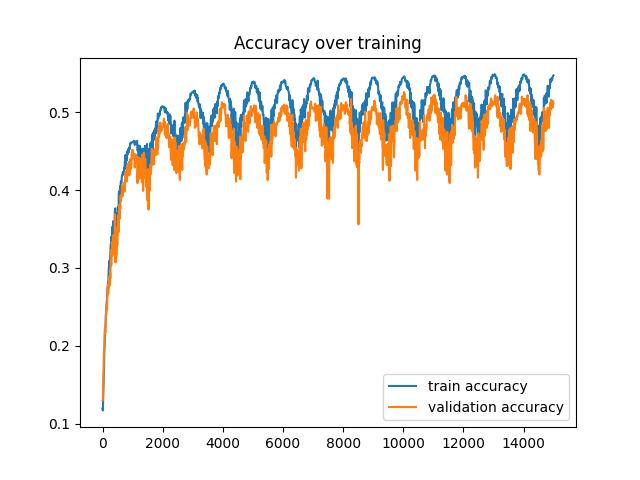
\includegraphics[width=\linewidth]{images/final_acc.png}
		\caption{Accuracy}
	\end{subfigure}
	\begin{subfigure}{0.3\textwidth}
		\centering
		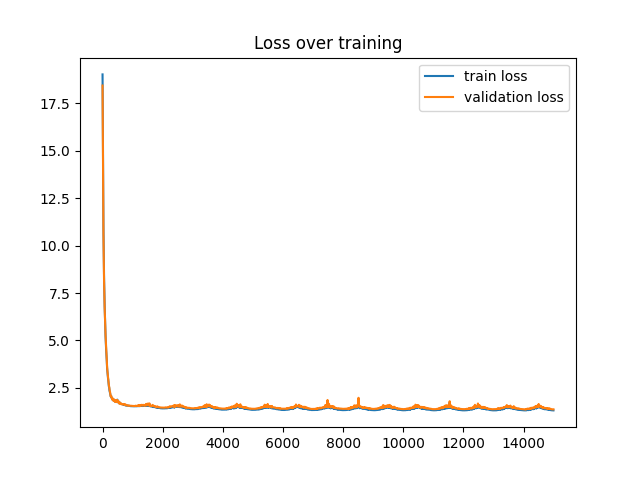
\includegraphics[width=\linewidth]{images/final_loss.png}
		\caption{Loss}
	\end{subfigure}
	\begin{subfigure}{0.3\textwidth}
		\centering
		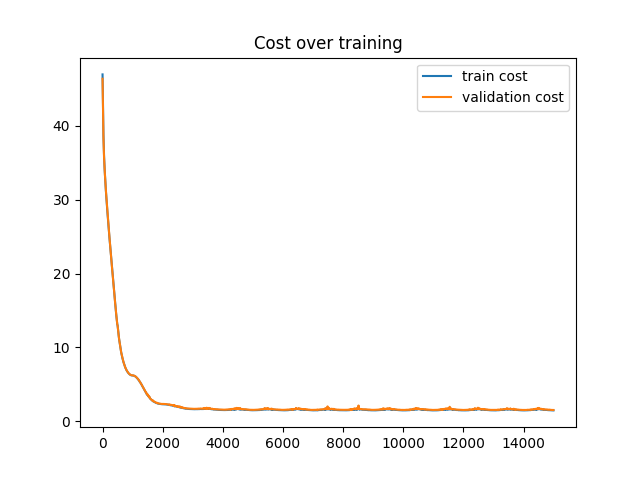
\includegraphics[width=\linewidth]{images/final_cost.png}
		\caption{Cost}
	\end{subfigure}
	\caption{Training of the final model with $\lambda=0.008$.}
	\label{fig:final}
\end{figure}


\section{Code explanation}
The code for this assignment has a very similar structure to the first assignment. Only a function for learning rate scheduling and some others for fine-tuning the parameters were added.

%%%%%%%% EXTRA TIPS %%%%%%%%
%% If you want to include an figure
%%\begin{figure}[H]
%%\includegraphics[]{Pendulum.jpg}
%%\caption{Sketch of the pendulum}
%%\label{fig:pendulum}
%%\end{figure}

%% for multiple figures in one fig
%\begin{figure}[h]
%	\centering
%	\begin{subfigure}{\textwidth}
%		\centering
%		\includegraphics[width=\linewidth]{images/sthfivo.png}
%		\caption{}
%	\end{subfigure}
%	\begin{subfigure}{\textwidth}
%		\centering
%		\includegraphics[width=\linewidth]{images/sth.png}
%		\caption{}
%	\end{subfigure}
%	\begin{subfigure}{\textwidth}
%		\centering
%		\includegraphics[width=\linewidth]{images/sth.png}
%		\caption{}
%	\end{subfigure}
%	\caption{caption}
%	\label{fig:label}
%\end{figure}


%% You can then reference with \ref{fig:pendulum}


%%\newpage
%\bibliographystyle{apacite}
%\bibliography{ref.bib}

\end{document}